\documentclass{article}

% Packages
\usepackage{fullpage}
\usepackage{amssymb}
\usepackage{multicol}
\usepackage{amsmath}
\usepackage{amsfonts}
\usepackage{bm}
\usepackage{float}
\usepackage{tikz}
\usepackage{xcolor}
\usetikzlibrary{shapes.geometric, positioning, arrows, intersections, backgrounds,arrows.meta}
\usepackage{amsthm}
\usepackage{tcolorbox}
\usepackage{hyperref}
\hypersetup{
    colorlinks=true, %set true if you want colored links
    linktoc=all,     %set to all if you want both sections and subsections linked
    linkcolor=black,  %choose some color if you want links to stand out
}
\usepackage{esint}
\usepackage{tikz-3dplot}

\tikzset {b/.code = {\pgfsetadditionalshadetransform{ \pgftransformshift{\pgfpoint{0 bp } { 0 bp }  }  \pgftransformrotate{0 }  \pgftransformscale{2 }  }}}
\pgfdeclarehorizontalshading{a}{150bp}{rgb(0bp)=(1,1,1);
rgb(37.5bp)=(1,1,1);
rgb(45.427829197474885bp)=(0.88,0.88,0.88);
rgb(50bp)=(0.95,0.95,0.95);
rgb(62.5bp)=(0.96,0.96,0.96);
rgb(100bp)=(0.96,0.96,0.96)}
\tikzset{every picture/.style={line width=0.75pt}}

% Macros
\newcommand{\R}{\mathbb{R}}
\newcommand{\N}{\mathbb{N}}
\newcommand{\Q}{\mathbb{Q}}
\newcommand{\sub}{\subset}
\renewcommand{\vec}[1]{\underline{\textbf{#1}}}
\newcommand{\uvec}[1]{\hat{\underline{\textbf{#1}}}}
\newcommand{\veci}{\bm{\hat{\imath}}}
\newcommand{\vecj}{\bm{\hat{\jmath}}}
\newcommand{\veck}{\bm{\hat{k}}}
\newcommand{\vecn}{\underline{\mathbf{\hat{n}}}}
\newcommand{\e}{\varepsilon}
\renewcommand{\th}{\vartheta}
\newcommand{\de}{\delta}
\renewcommand{\k}{\kappa}
\newcommand{\p}{\Phi}
\newcommand{\pa}{\partial}
\newcommand{\kd}{\delta_{i, j}}
\newcommand{\at}{\e_{i, j, k}}
\newcommand{\nab}{\underline{\nabla}}
\newcommand{\grad}{{\nab}\, f}
\newcommand{\pd}[2]{\frac{\partial #1}{\partial #2}}
\newcommand{\fd}[2]{\frac{d #1}{d #2}}
\renewcommand{\div}{\nab \cdot}
\newcommand{\curl}{\nab \times}

%ToC stuff
\newtheorem{example}{Example}
\newtheorem{solution}{Solution}
%\newtheorem{definition}{Definition}[subsection]
\newtheorem{corollary}{Corollary}

\tcbuselibrary{theorems}
\newtcbtheorem[number within=section]{theorem}{Theorem}%
{colback=green!5,colframe=green!35!black,fonttitle=\bfseries}{th}
\newtcbtheorem[number within=section]{definition}{Definition}%
{colback=blue!5,colframe=blue!35!black,fonttitle=\bfseries}{def}

\title{Vector Calculus Week 4 - Vector Operators}
\author{James Arthur}

\begin{document}
\maketitle
\tableofcontents\newpage

\multicols{2}

\section{Conservative Fields}
\subsection{Gradients and Conserivative Field}

\begin{figure}[H]
  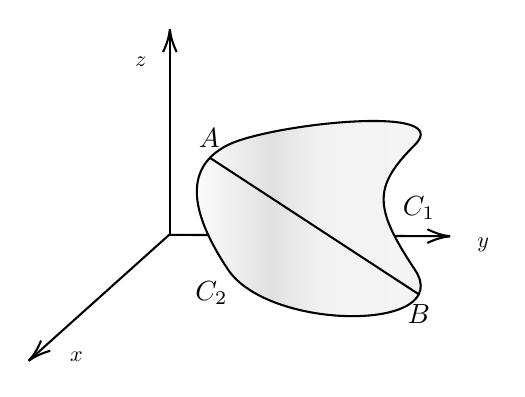
\begin{tikzpicture}[x=0.75pt,y=0.75pt,yscale=-1,xscale=1]
  \draw    (180,111) -- (112,172) ; % x axis
  \draw [shift={(112,172)}, rotate = 318.26] [color=black]   (0,0) .. controls (3.31,-0.3) and (6.95,-1.4) .. (10.93,-3.3)(0,0) .. controls (3.31,0.3) and (6.95,1.4) .. (10.93,3.29)   ; % x axis arrow

  \draw    (180,111) -- (180,12) ; % axis
  \draw [shift={(180,12.32)}, rotate = 450] [color=black]   (0,0) .. controls (3.31,-0.3) and (6.95,-1.4) .. (10.93,-3.29)(0,0) .. controls (3.31,0.3) and (6.95,1.4) .. (10.93,3.29)   ;

  \draw    (180,111.32) -- (315,112) ; %axis
  \draw [shift={(315,112)}, rotate = 180.42] [color=black]   (0,0) .. controls (3.31,-0.3) and (6.95,-1.4) .. (10.93,-3.29)(0,0) .. controls (3.31,0.3) and (6.95,1.4) .. (10.93,3.29)   ;

  \path  [shading=a,b] (208,68) .. controls (228,58) and (318,48) .. (298,68) .. controls (278,88) and (278,98) .. (298,128) .. controls (318,158) and (228,158) .. (208,128) .. controls (188,98) and (188,78) .. (208,68) ; % fills path
   \draw   (208,68) .. controls (228,58) and (318,48) .. (298,68) .. controls (278,88) and (278,98) .. (298,128) .. controls (318,158) and (228,158) .. (208,128) .. controls (188,98) and (188,78) .. (208,68) ; % draws outline

  \draw (199,74) node [above] {$A$} -- (300,140) node [below] {$B$}; % draws line

  \draw (200,150) node [above] {$C_2$};
  \draw (300,88) node [below] {$C_1$};
  \draw (135,170) node [scale=0.8]  {$x$};
  \draw (331,116) node [scale=0.8]  {$y$};
  \draw (166,28) node [scale=0.8]  {$z$};
  \end{tikzpicture}
\end{figure}

\noindent\begin{definition}{Conservative Vector Field}{}
 A conservative vector field is one which the line integral along a curve connecting two points does not depend on the path taken.
\end{definition}\vspace{10pt}

What this says, is that we can write:
$$ \int_{C} {\vec F \cdot d\vec r} = \int_{C_1}{\vec F \cdot d\vec r} = \int_{C_2}{\vec F \cdot d\vec r} $$

\noindent\begin{theorem}{}{}
 Suppose that a vector field $\vec F$ is related to a scalar field $\p (\vec x)$ by $\displaystyle{\vec F = \nab \p}$ and $\nab\p$ exists everywhere in some region $D$. Conversely, if $\vec F$ is conservative, then $\vec F$ can be written as the gradient of a scalar field, $\displaystyle{\vec F = \nab\p}$
\end{theorem}\vspace{10pt}
\begin{proof}
  Suppose that $\displaystyle{\vec F = \nab\p}$, then $F$ is conservative on $D$. So we can write;
  \begin{align*}
     \int_C {\vec F \cdot d\vec r} &= \int_C {\nab\p \cdot d\vec r}\\
     &= \int_C \left( \pd{\p}{x}, \pd{\p}{y}, \pd{\p}{z} \right)\cdot\left(dx,dy, dz\right)\\
     &= \int_C \pd{\p}{x}dx + \pd{\p}{y}dy + \pd{\p}{z}dz\\
     &= \int_C d\p\\
   \end{align*}
   \begin{align*}
     &= \p\Bigr|_A^B \\
     &= \p(B) - \p(A)\\
  \end{align*}
  So as this result only matters about the end points, $\vec F$ is conservative. Now assume that $\vec F$ is conservative, then a scalar field $\p(\vec x)$ can be defined as the line integral of $\vec F$ from the origin to the point $\vec x$:
  \begin{align*}
    \p(\vec x) &= \int_{\vec 0}^{\vec x}{\vec F \cdot d\vec r}\\
    d\p &= \vec F \cdot d\vec r \\
    &= \nab\p \cdot \vec r \\
    &= \pd{\p}{x}dx +\pd{\p}{y}dy + \pd{\p}{z}dz
  \end{align*}
  and we can now say that $\displaystyle{\vec F \cdot d\vec r = \nab\p \cdot d\vec r}$ and hence, $F = \nab\p$
\end{proof}

If a vector field is conservative, $\p(\vec x)$ which satisfies $\vec F = \nab \p$ is called the potential of the vector field.

\subsection{Curl and conservative vector fields}
Suppose that $\displaystyle{\vec u = \nab\p}$, then,
\begin{align*}
  \curl\vec u &= \left( \pd{}{x}, \pd{}{y}, \pd{}{z}\right)\times (u_1, u_2, u_3)\\
  &= \left|\begin{matrix}
    \veci & \vecj & \veck \\
    \pd{}{x} & \pd{}{y} & \pd{}{z} \\
    u_1 & u_2 & u_3 \\
  \end{matrix}\right|\\
  &= \left( \pd{u_3}{y} - \pd{u_2}{z} \right)\veci + \left(\pd{u_1}{z} - \pd{u_3}{z}\right)\vecj + \left(\pd{u_2}{x} - \pd{u_1}{y} \right)\veck\\
  &= \left(\pd{^2\p}{y\pa z}- \pd{^2\p}{z\pa y} \right)\veci \left(\pd{^2\p}{z\pa x} - \pd{^2\p}{x\pa z} \right)\vecj \\
  &\quad+ \left(\pd{^2\p}{x \pa y} - \pd{^2\p}{y\pa x}\right)\veck\\
  &= \vec 0 \qquad\text{As $\p \in C^2$}
\end{align*}
So for any vector $\vec u$ that can be written as the gradient of a vector field is irrotational. Conversely, any irrotational vector field is conservative.

\subsection{Laplacian of a scalar field}
 Suppose that a scalar field $\p$, is twice dofferenctiable. Then $\nab\p$ is a differentiable vector field, so we can tak divergence of $\nab\p$ and obtain another scalar field\\
\noindent\begin{definition}{Laplacian}{}
 The scalar field $\div\nab\p$ is called the Laplacian of $\p$ and is denoted, $\nabla^2$ or $\Delta$
\end{definition}\vspace{10pt}

The Laplacian can also act on a vector field, which results in another vector field.
\begin{align*}
  \nabla^2\vec u &= {\nabla^2 u}_1 \veci + {\nabla^2 u}_2 \vecj + {\nabla^2 u}_3 \veck
\end{align*}
If we have $\Delta \p = 0$, this is a known PDE known as the laplace equation.

\noindent\begin{theorem}{Divergence of curl}{}
 For any $\mathcal{C}^2$ vector field, $\vec F$,
 $$ \div \curl \vec F = 0 $$
\end{theorem}\vspace{10pt}
\begin{proof}
  \begin{align*}
    \curl \vec F &= \left|\begin{matrix}
      \veci & \vecj & \veck \\
      \pd{}{x} & \pd{}{y} & \pd{}{z} \\
      F_1 & F_2 & F_3 \\
    \end{matrix}\right|\\
  &= \left( \pd{F_3}{y} - \pd{F_2}{z} \right)\veci +\\
  &\quad \left(\pd{F_1}{z} - \pd{F_3}{z}\right)\vecj + \left(\pd{F_2}{x} - \pd{F_1}{y} \right)\veck\\
  \div\curl\vec F &= \pd{F_3}{x\pa y} - \pd{F_2}{x\pa z}+ \pd{F_1}{y \pa z}\\
  &\quad- \pd{F_3}{x \pa y} + \pd{F_2}{x \pa z} - \pd{F_1}{y \pa z}\\
  &= \vec 0
  \end{align*}
\end{proof}

\subsection{Vector Operators Identities}
Let $\p, f, g$ be scalar fields and $\vec F, \vec G$ be vector fields, then:

\begin{align}
  \div(\curl\vec F) &= 0\\
  \curl\nab\p &= \vec 0\\
  \nab(f + g) &= \grad + \nab g\\
  \div(\vec F + \vec G) &= \div\vec F + \div\vec G \\
  \curl(\vec F + \vec G) &= \curl\vec F + \curl\vec G\\
  \nab(fg) &= f\nab g + g\nab f\\
  \div(\p\vec F) &= \p\div\vec F + \vec F \cdot \nab\p\\
  \curl(\p\vec F) &= \p\curl\vec F - \vec F\times\nab\p \\
  \nab(\vec F \cdot\vec G) &= \vec F\times(\curl \vec G) + \vec G\times(\curl \vec F) \\
  &\quad + (\vec F \cdot\nab)\vec G + (\vec G \cdot \nab)\vec F\\
\end{align}

\begin{align}
  \div(\vec F\times \vec G) &= \vec G \cdot(\curl\vec F) - \vec F(\curl \vec G)\\
  \curl(\vec F\times \vec G) &= \vec F(\div \vec G) - \vec G(\div \vec F)\\
  &\quad + (\vec G \cdot\nab)\vec F - (\vec F \cdot\nab)\vec G\\
  \curl(\curl\vec F) &= \nab(\div\vec F) - \nab^2\vec F
\end{align}


\section{Orthoginal Curvilinear Co-ordinate Systems}
Assume a one to one map from $x_i$ to $u_i$, the surfaces $u_i = k$ are defined as a co-ordinate surface and the intersection of the co-ordinate curves.
$$ d\vec r = (dx_1, dx_2, dx_3) = \pd{\vec r}{u_1} du_1 + \pd{\vec r}{u_2}du_2 + \pd{\vec r}{u_3}du_3 $$

\begin{figure}[H]
  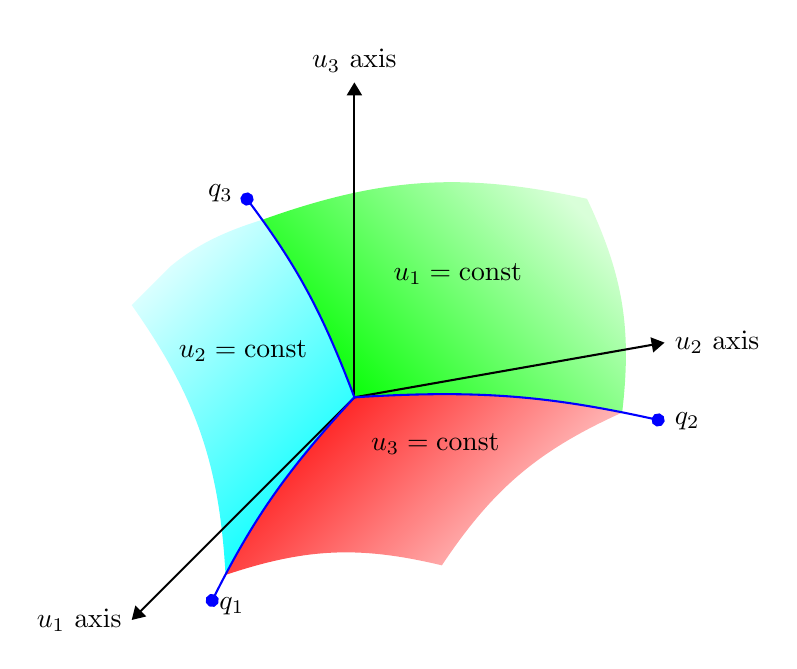
\begin{tikzpicture}[x=(10:4cm),y=(90:4cm),z=(225:4cm),>=Triangle]
  \coordinate (O) at (0,0,0);
  \draw [->] (O) -- (1,0,0) node [at end, right] {$u_2$ axis};
  \draw [->] (O) -- (0,1,0) node [at end, above] {$u_3$ axis};
  \draw [->] (O) -- (0,0,1) node [at end, left]  {$u_1$ axis};

  \draw [draw=blue, -Circle] (O) to [bend left=8]
    coordinate [pos=7/8] (q2n)
    (1,-1/4,0) coordinate (q2) node [right] {$q_2$};
  \draw [draw=blue, -Circle] (O) to [bend right=8]
    coordinate [pos=7/8] (q3n)
    (0,1,1/2) coordinate (q3) node [left] {$q_3$};
  \draw [draw=blue, -Circle] (O) to [bend right=8]
    coordinate [pos=7/8] (q1n)
    (1/4,0,1) coordinate (q1) node [right] {$q_1$};

  \begin{pgfonlayer}{background}
  \begin{scope}
  \clip (O) to [bend left=8] (q2) -- (1,1,0) -- (q3n) to [bend right=8] (O);
  \shade [left color=green, right color=green!15!white, shading angle=135]
    (O) to [bend left] (q3n) to [bend left=16] (3/4,1/2,0) to [bend left=16] (q2n) -- cycle;
  \end{scope}

  \begin{scope}
  \clip (O) to [bend left=8] (q2) -- (1,0,1) -- (q1) to [bend left=8] (O);
  \shade [left color=red, right color=red!15!white, shading angle=45]
    (O) to [bend right] (q1n) to [bend left=16] (1,0,1) to [bend left=16]
    (q2n) to [bend right] (O);
  \end{scope}

  \begin{scope}
  \clip (O) to [bend right=8] (q1) -- (0,1,1) -- (q3) to [bend left=8] (O);
  \shade [left color=cyan, right color=cyan!15!white, shading angle=225]
    (O) -- (q1n) to [bend right=16] (0,1,1) to [bend left=16] (q3n)
  to [bend left] (O);
  \end{scope}
  \end{pgfonlayer}

  \node at (1/3,1/3,0) {$u_1=\mbox{const}$};
  \node at (0,1/2,1/2) {$u_2=\mbox{const}$};
  \node at (1/2,0,1/3) {$u_3=\mbox{const}$};
  \end{tikzpicture}
\end{figure}

\subsection{Scale Factors}

If we let $\vec e_1$ be an arbitrary unit vector in the direction of $u_1$, and similarly for $\vec e_2$ and $\vec e_3$, then:
$$ e_1 = \pd{\vec r}{u_1}\frac{1}{h_1} \qquad h_1 = \left|\pd{\vec r}{u_1} \right| $$
and similarly for $\vec e_2$ and $\vec e_3$. Now we can rewrite $d\vec r$:
$$ d\vec r = h_1\vec e_1 du_1 + h_2\vec e_2 du_2 + h_3\vec e_3 du_3 $$
We want, $\vec e_i \cdot \vec e_j = \delta_{ij}$ and $(\vec e_1, \vec e_2, \vec e_3)$ to be right handed.

\subsection{Differential of arc length}
Let $\displaystyle{d\vec r} = h_1du_1\vec e_1 + h_2du_2\vec e_2 + h_3du_3\vec e_3$, then, $\displaystyle{ds^2 = h_1^2du_1^2 + h_2du_2^2 + h_3^2du_3^2}$. Now we find $dS$, by taking the pross product between $\displaystyle{\pd{\vec r}{u_1}u_1}$ and $\displaystyle{\pd{\vec r}{u_3}du_3}$. Hence for $u_1$ surface,
$dS = h_2h_3du_2du_3$
for the u_2 surfa


\subsection{Grad, Curl and Div in Curvilinear Co-ordinates}


\subsection{Cylindrical and Spherical Co-ordinate Systems}










\end{document}
